 \documentclass[11pt]{amsart}


\usepackage[all]{xy}
\usepackage{graphics}
\graphicspath{./images/}
\usepackage{enumitem}
\usepackage{epsfig}
\usepackage{amsmath}
\usepackage{amscd}
\usepackage{tikz-cd}
\usepackage{verbatim}
\usepackage{pdfpages}
%\usepackage{showkeys}
\usepackage{amsfonts,latexsym,amssymb}
\usepackage{parskip}
\usepackage{MnSymbol}
\usepackage{hyperref}

\usepackage{mdwlist}



%%%%%%%%%%%%%%%%%%%%%%%%%%%%%%%%%%%%%%%%%%%%%%%%%%%%%%%%


\newcommand{\cA}{{\mathcal{A}}}   \newcommand{\cB}{{\mathcal{B}}}
\newcommand{\cC}{{\mathcal{C}}}   \newcommand{\cD}{{\mathcal{D}}}
\newcommand{\cE}{{\mathcal{E}}}   \newcommand{\cF}{{\mathcal{F}}}
\newcommand{\cG}{{\mathcal{G}}}   \newcommand{\cH}{{\mathcal{H}}}
\newcommand{\cI}{{\mathcal{I}}}   \newcommand{\cJ}{{\mathcal{J}}}
\newcommand{\cK}{{\mathcal{K}}}   \newcommand{\cL}{{\mathcal{L}}}
\newcommand{\cM}{{\mathcal{M}}}   \newcommand{\cN}{{\mathcal{N}}}
\newcommand{\cO}{{\mathcal{O}}}   \newcommand{\cP}{{\mathcal{P}}}
\newcommand{\cQ}{{\mathcal{Q}}}   \newcommand{\cR}{{\mathcal{R}}}
\newcommand{\cS}{{\mathcal{S}}}   \newcommand{\cT}{{\mathcal{T}}}
\newcommand{\cU}{{\mathcal{U}}}   \newcommand{\cV}{{\mathcal{V}}}
\newcommand{\cW}{{\mathcal{W}}}   \newcommand{\cX}{{\mathcal{X}}}
\newcommand{\cY}{{\mathcal{Y}}}   \newcommand{\cZ}{{\mathcal{Z}}}

\newcommand{\hcP}{\hat{\mathcal{P}}}
\newcommand{\hcQ}{\hat{\mathcal{Q}}}
\newcommand{\hcR}{\hat{\mathcal{R}}}
\newcommand{\hcL}{\hat{\mathcal{L}}}
\newcommand{\hcM}{\hat{\mathcal{M}}} \newcommand{\hphi}{\hat{\phi}}
\newcommand{\bbk}{\mathbb{k}}   \newcommand{\bfv}{\mathbf{v}}
\newcommand{\bfnu}{\mathbf{nu}}  \newcommand{\hXX}{\hat{\mathbb{X}}}
\newcommand{\bJ}{\mathbf{J}}

\newcommand{\hD}{{\hat{D}}}   \newcommand{\hE}{{\hat{E}}}
\newcommand{\hF}{{\hat{F}}}   \newcommand{\hH}{{\hat{H}}}
\newcommand{\hY}{{\hat{Y}}}   \newcommand{\hP}{{\hat{P}}}
\newcommand{\hT}{{\hat{T}}}   \newcommand{\hQ}{{\hat{Q}}}
\newcommand{\hq}{{\hat{q}}}
\newcommand{\hr}{{\hat{r}}}
\newcommand{\hu}{{\hat{u}}}
\newcommand{\hv}{{\hat{v}}}
\newcommand{\hf}{{\hat{f}}}
\newcommand{\hg}{{\hat{g}}}
\newcommand{\hw}{{\hat{w}}}
\newcommand{\hS}{{\hat{S}}}
\newcommand{\hV}{{\hat{V}}}
\newcommand{\hG}{{\hat{G}}}
\newcommand{\hmu}{{\hat{\mu}}}
\newcommand {\y}{\V{y}}
\newcommand {\V}[1]{\mbox{\boldmath$#1$}}
\newcommand{\iExp}{{\mathrm{iExp\,}}}

\newcommand{\htheta}{{\hat{\theta}}}



\newcommand{\htu}{{\hat{\tilde{u}}}}


\newcommand{\hTR}{{\widehat{TR}}}
\newcommand{\tsigma}{{\tilde{\sigma}}}
\newcommand{\tphi}{{\tilde{\phi}}}
\newcommand{\tpsi}{{\tilde{\psi}}}
\newcommand{\tzeta}{{\tilde{\zeta}}}
\newcommand{\tdelta}{{\tilde{\delta}}}
\newcommand{\tgamma}{{\tilde{\gamma}}}
\newcommand{\tGamma}{{\tilde{\Gamma}}}
\newcommand{\tlog}{{\widetilde{\log}}}


\newcommand{\txi}{{\tilde{\xi}}}
\newcommand{\tomega}{{\tilde{\omega}}}
\newcommand{\tH}{{\tilde{H}}}
\newcommand{\tI}{{\tilde{I}}}

\newcommand{\tX}{{\tilde{X}}}
\newcommand{\tV}{{\tilde{V}}}
\newcommand{\tz}{{\tilde{z}}}
\newcommand{\ty}{{\tilde{y}}}
\newcommand{\tx}{{\tilde{x}}}
\newcommand{\te}{{\tilde{e}}}
\newcommand{\tf}{{\tilde{f}}}
\newcommand{\tg}{{\tilde{g}}}
\newcommand{\tu}{{\tilde{u}}}
\newcommand{\tm}{{\tilde{m}}}
\newcommand{\tn}{{\tilde{n}}}
\newcommand{\tilt}{{\tilde{t}}}
\newcommand{\tT}{{\tilde{T}}}
\newcommand{\tL}{{\tilde{L}}}
\newcommand{\tQ}{{\tilde{Q}}}
\newcommand{\tB}{{\tilde{B}}}
\newcommand{\tC}{{\tilde{C}}}
\newcommand{\tD}{{\tilde{D}}}
\newcommand{\tU}{{\tilde{U}}}
\newcommand{\utL}{{\underline{\tilde{L}}}}
\newcommand{\tF}{{\tilde{F}}}\newcommand{\tilh}{{\tilde{h}}}
\newcommand{\tk}{{\tilde{k}}}
\newcommand{\tv}{{\tilde{v}}}
\newcommand{\tw}{{\tilde{w}}}
\newcommand{\bx}{\mathbf x}
\newcommand{\bz}{\mathbf z}
\newcommand{\bu}{\mathbf u}
\newcommand{\bv}{\mathbf v}
\newcommand{\bt}{\mathbf t}
\newcommand{\bi}{\mathbf i}
\newcommand{\bj}{\mathbf j}
\newcommand{\bL}{\mathbf L}
\newcommand{\bN}{\mathbf N}
\newcommand{\bM}{\mathbf M}
\newcommand{\bB}{\mathbf B}
\newcommand{\bA}{\mathbf A}
\newcommand{\tbz}{{\tilde{\mathbf z}}}
\newcommand{\hbx}{\hat{\mathbf x}}
\newcommand{\tcO}{{\tilde{\mathcal{O}}}}
\newcommand{\tcC}{{\tilde{\mathcal{C}}}}
\newcommand{\ocC}{{\overline{\mathcal{C}}}}
\newcommand{\tcR}{{\tilde{\mathcal{R}}}}
\newcommand{\tcA}{{\tilde{\mathcal{A}}}}








\newcommand{\uL}{\underline L}
\newcommand{\uM}{\underline M}
\newcommand{\uE}{\underline E}

\newcommand{\chA}{\check A}
\newcommand{\chE}{\check E}
\newcommand{\chL}{\check L}
\newcommand{\chV}{\check V}
\newcommand{\chv}{\check v}
\newcommand{\chw}{\check w}
\newcommand{\chW}{\check W}
\newcommand{\chM}{\check M}
\newcommand{\chQ}{\check Q}
\newcommand{\chsigma}{\check\sigma}



\newcommand{\uchL}{\underline{\check L}}






\newcommand{\BA}{\mathbb{A}}  \newcommand{\BB}{\mathbb{B}}
\newcommand{\CC}{\mathbb{C}}  \newcommand{\EE}{\mathbb{E}}
\newcommand{\FF}{\mathbb{F}}  \newcommand{\HH}{\mathbb{H}}
\newcommand{\JJ}{\mathbb{J}}  \newcommand{\LL}{\mathbb{L}}
\newcommand{\NN}{\mathbb{N}}  \newcommand{\PP}{\mathbb{P}}
\newcommand{\QQ}{\mathbb{Q}}  \newcommand{\RR}{\mathbb{R}}
\newcommand{\TT}{\mathbb{T}}  \newcommand{\VV}{\mathbb{V}}
\newcommand{\XX}{\mathbb{X}}  \newcommand{\WW}{\mathbb{W}}
\newcommand{\ZZ}{\mathbb{Z}}

\newcommand{\FM}{\mathfrak{M}}
\newcommand{\fm}{\mathfrak{m}}


\newcommand{\isom}{\cong}
\newcommand{\Ext}{\operatorname{Ext}}
\newcommand{\Grass}{\operatorname{Grass}}
\newcommand{\coker}{\operatorname{coker}}
\newcommand{\Hilb}{\operatorname{Hilb}}
\newcommand{\Hom}{\operatorname{Hom}}
\newcommand{\Quot}{\operatorname{Quot}}
\newcommand{\Pic}{\operatorname{Pic}}
\newcommand{\NS}{\operatorname{NS}}
\newcommand{\Sym}{\operatorname{Sym}}
\newcommand{\id}{\operatorname{I}}
\newcommand{\im}{\operatorname{im}}
\newcommand{\surj}{\twoheadrightarrow}
\newcommand{\inj}{\hookrightarrow}
\newcommand{\gr}{\operatorname{gr}}
\newcommand{\rk}{\operatorname{rk}}
\newcommand{\reg}{\operatorname{reg}}
\newcommand{\wt}{\widetilde}
\newcommand{\del}{{\partial}}
\newcommand{\delb}{{\overline\partial}}

\newcommand{\oX}{{\overline X}}
\newcommand{\oD}{{\overline D}}
\newcommand{\ox}{{\overline x}}
\newcommand{\ow}{{\overline w}}
\newcommand{\oz}{{\overline z}}
\newcommand{\oh}{{\overline{h}}}
\newcommand{\oalpha}{{\overline \alpha}}





\newcommand{\Res}{\operatorname{Res}}
\newcommand{\ch}{\operatorname{ch}}
\newcommand{\tr}{\operatorname{tr}}
\newcommand{\pardeg}{\operatorname{par-deg}}
\newcommand{\ad}{{ad\,}}
\newcommand{\diag}{\operatorname{diag}}
\newcommand{\codim}{\operatorname{codim}}

\hyphenation{pa-ra-bo-lic}
\newcommand{\bbQ}{\mathbb{Q}}
\newcommand{\bbR}{\mathbb{R}}
\newcommand{\bbP}{\mathbb{P}}
\newcommand{\bbC}{\mathbb{C}}
\newcommand{\bbT}{\mathbb{T}}
\newcommand{\bbU}{\mathbb{U}}
\newcommand{\bbZ}{\mathbb{Z}}
\newcommand{\bbN}{\mathbb{N}}
\newcommand{\bbF}{\mathbb{F}}






\newtheorem{proposition}{Proposition}[section]
\newtheorem{theorem}[proposition]{Theorem}
\newtheorem{lemma}[proposition]{Lemma}
\newtheorem{conjecture}[proposition]{Conjecture}
\newtheorem{corollary}[proposition]{Corollary}


\theoremstyle{definition}
\newtheorem{definition}[proposition]{Definition}
\newtheorem{remark}[proposition]{Remark}
\newtheorem{notation}[proposition]{Notation}
\newtheorem{example}[proposition]{Example}
\newtheorem{ex}{Exercise}[section]
 

%%%%%%%%%%%%%%%%%%%%%%%%%%%%%%%%%%%%%%%%%%%%%%%%%%%%%%%%

\begin{document}

\title{CMI UG Calculus 2020 Assignment 2\\
 {\tiny Higher-dimensional Riemann integrals, \underline{due 10 September}}}
\author{Sampad Kumar Kar -- BMC201944}
\date{\today}
\maketitle

\begin{enumerate}[wide, labelwidth=!, labelindent=0pt]

\item  In my class notes I made the claim: ``Lower Riemann sums increase under refinement and upper Riemann sums decrease under refinement." Formulate this in ``notational" terms and prove it.

\textbf{Solution 1:}

Let $f$ be a real valued, bounded function on $[a,b]$.
Let $P = \{x_0,x_1,...,x_n\}$ be a partition of $[a,b]$ and let $Q$ be a refinement of $P$. So, we have to show that $L(P,f)\le L(Q,f)$ and $U(P,f) \ge U(Q,f)$.

First, I will show what happens when we refine $P$ by just one additional point $y$ to some sub-interval, say $[x_{t-1},x_t]$ of $P$ to the lower sum. Let $m_t = inf \{f(x) | x \in [x_{k-1},x_k]\}$ for each sub interval of $P$. Then we have-
$$m_t(x_t - x_{t-1}) = m_t(x_t - y) + m_t(y - x_{t-1}) \le m_t '(x_t - y) + m_t ''(y - x_{t-1})$$ where
$$m_t' = inf \{f(x) | x \in [x_{k-1},y]\}$$ and $$m_t'' = inf \{f(x) | x \in [y,x_k]\}$$ as each $m_t'$ and $m_t''$ are respectively greater than or equal to $m_t$. As the remaining sub intervals still give the same sum, we conclude that the total lower sum of $P$ is less than that of $Q$.

Now, if $Q$ differs from $P$ by some $m$ points, we repeat this process $m$ times, in the respective sub interval, and each time it will result in increase in the lower sum. Hence, $L(P,f)\le L(Q,f)$.

An analogous argument holds for upper sums when we take the supremum in the sub intervals containing refinement points in $P$ showing that $U(P,f) \ge U(Q,f)$.

\newpage
\item A real-valued function $f$ on an interval $I$ is \emph{monotone} if it is either non-increasing or non-decreasing. Prove that if $I$ is closed and bounded and a function $f$ is monotone, then $f$ is integrable.

\textbf{Solution 2:}

Without loss of generality, assume $f$ is monotonically increasing on the interval $[a,b]$. Consider an $\epsilon > 0$. We will construct a partition $P$ of $[a,b]$ such that $U(P,f) - L(P,f) < \epsilon$.

Since $f$ is monotonically increasing on $[a,b] \implies f(a) \le f(b)$. First, we consider the case when $f(a) = f(b)$. Then clearly $f$ is a constant function, and hence Riemann integrable. Now consider when $f(a) < f(b)$. Consider, $k$ such that $k(f(b)-f(a)) < \epsilon$. Such a $k$ will exist because $f$ is bounded.

Now, divide the interval $[a,b]$ in $\lfloor \frac{b-a}{k} \rfloor + 1$ number of sub intervals of equal length, such that length of each sub interval is less than $k$. Let this partition be $P = \{x_0, x_1,...,x_{n}\}$.

Now, in each sub interval $[x_{t-1},x_t]$, due to monotonicity of $f$, $m_t = f(x_{t-1})$ and $M_t = f(x_t)$. Thus we have - $$U(P,f)-L(P,f) = \sum_{t=1}^{t=n} (M_t - m_t)(x_t - x_{t-1}) = \sum_{t=1}^{t=n} (f(x_t) - f(x_{t-1}))(x_t - x_{t-1})$$ $$ < \sum_{t=1}^{t=2k} (f(x_t) - f(x_{t-1}))k = k\sum_{t=1}^{t=2k} (f(x_t) - f(x_{t-1})) = k(f(b)-f(a)) < \epsilon$$

Hence, $f$ is Riemann integrable.

\newpage
Now we move to higher dimensions.

\item \texttt{[This carries no marks; do not submit a solution]} In the notes we have a priori two definitions for the area of a rectangle $R=[a_1,b_1] \times [a_2,b_2]$: $area(R)=(b_2-a_2)(b_1-a_1)$ and
$$
area(R)=\int_R \mathbf{1} dx
$$
Check that the two coincide.

\item Let $X$ be a metric space and $E$ a subset. Prove that $\partial E=\partial E^c$.

\textbf{Solution 4:}

We know that $\partial E = \overline{E}-E^o = \overline{E} \cap (E^o)^c$. This means $\partial E^c = \overline{E^c} - (E^c)^o$.

\textit{Claim:} $(\overline{E})^c = (E^c)^o$.

\textit{Proof:} Let $x\in (\overline{E})^c \implies x \in E^c$. As $x \notin \overline{E}, \exists \epsilon > 0, B(x,\epsilon) \cap E = \phi \implies B(x,\epsilon) \subseteq E^c \implies x \in (E^c)^o \implies (\overline{E})^c \subseteq (E^c)^o$.

Let $x\in (E^c)^o \implies \exists \epsilon >0, B(x,\epsilon) \subseteq E^c \implies x \notin E \implies x \notin \overline{E} \implies x \in (\overline{E})^c \implies (E^c)^o \subseteq (\overline{E})^c$.

Hence, $(\overline{E})^c = (E^c)^o$.

Using the above result, $(\overline{E^c})^c = ((E^c)^c)^o \implies (\overline{E^c})^c = E^o \implies \overline{E^c} = (E^o)^c$.

Now, $\partial E = \overline{E}-E^o = \overline{E} \cap (E^o)^c = \overline{E} \cap \overline{E^c} \implies \partial E = \overline{E} \cap \overline{E^c}$. 

This means $\partial E = \overline{E} \cap \overline{E^c} = \partial E^c$. Hence, we are done.

\newpage
\item Let $T \subset \bbR^2$ be a compact  subset with content zero. Show that $T$ is acceptable, and $area(T)=0$.

Hint: Argue that $\partial T \subset T$ so $\partial T$ has content zero. So $T$ is acceptable.

\textbf{Solution 5:}

We know that $T$ is acceptable iff $\partial T$ has content zero. Given, $T$ is compact with content zero. As $T$ is compact, it is closed and bounded. Since it is closed, $\overline{T} = T$. Now $\partial T = \overline{T}-T^o = T-T^o \implies \partial T \subseteq T$.

Consider any $\epsilon > 0$. As $T$ has content zero, $\exists$ a collection of closed rectangles $R_1, R_2,...R_n$ such that $\partial T \subseteq T \subseteq \cup_{i = 1}^{n} R_i$ and $\sum_{i=1}^{n} \text{area}(R_i) < \epsilon$. This means $\partial T$ also has content zero, which means $T$ is acceptable.

\textit{Claim 1:} If $A$ and $B$ are acceptable, then $A \cup B$ is also acceptable.

\textit{Proof:} Let $S = A \cup B$. In order to show this, it is enough to show that $\partial S \subseteq \partial A \cup \partial B$.

Now, $\partial S = \overline{S} \cap \overline{S^c} = \overline{A \cup B} \cap \overline{(A \cup B)^c} = \overline{A \cup B} \cap \overline{A^c \cap B^c} = (\overline{A} \cup \overline{B}) \cap \overline{A^c \cap B^c} = (\overline{A} \cap \overline{A^c \cap B^c}) \cup (\overline{B} \cap \overline{A^c \cap B^c}) \subseteq (\overline{A} \cap (\overline{A^c} \cap \overline{B^c})) \cup (\overline{B} \cap (\overline{A^c} \cap \overline{B^c})) = ((\overline{A} \cap \overline{A^c}) \cap (\overline{B} \cap \overline{B^c})) \cup ((\overline{B} \cap \overline{A^c}) \cap (\overline{B} \cap \overline{B^c})) \subseteq (\overline{A} \cap \overline{A^c}) \cup (\overline{B} \cap \overline{B^c}) = \partial A \cup \partial B$.

Now, as $A$ and $B$ are acceptable, $\partial A$ and $\partial B$ have content zero. And as shown in class, the union of $2$ sets with content zero, also has content zero. So, $\partial A \cup \partial B$ also has content zero. Now, following the arguments in previous part, where we showed, that subsets of content zero sets also have content zero, $\partial S \subseteq \partial A \cup \partial B$ also has content zero, implying, $S = A \cup B$ is acceptable.

\textit{Claim 2:} $area(R_1 U R_2) \le area(R_1) + area(R_2)$.

\textit{Proof:} Now, $R_1$ and $R_2$ are trivially acceptable. So, $S = R_1 \cup R_2$ is also acceptable by \textbf{Claim 1}.

If $R_1$ and $R_2$ are disjoint, then as we proved in class that $area(S) = $ $area(R_1) + area(R_2)$. Suppose they are not disjoint, then consider $\chi_{S}, \chi_{R_1}$ and $\chi_{R_2}$, with respect to the closed rectangle $R$ containing $S, R_1$ and $R_2$ (closed rectangle containing $R$ will contain $R_1$ and $R_2$ as well).

Notice, let $g = \chi_{R_1} + \chi_{R_2}$.
Now,
\[
g(x) = 
\begin{cases} 
      1 & x\in R_1 \Delta R_2 \\
      2 & x\in R_1 \cap R_2 \\
      0 & x \in R-S\\
\end{cases}
\]
and as $S = R_1 \cup R_2 = (R_1 \Delta R_2) \cup (R_1 \cap R_2)$
\[
\chi_{S}(x) = 
\begin{cases} 
      1 & x\in R_1 \Delta R_2 \\
      1 & x\in R_1 \cap R_2 \\
      0 & x \in R-S\\
\end{cases}
\]
Clearly, $\chi_S(x) \le g(x)$ $\forall x \in R$. Hence, $area(S) = \int_{x \in R} \chi_S(x) dx \le \int_{x \in R} g(x) dx = \int_{x \in R} (\chi_{R_1}(x) + \chi_{R_2}(x)) dx = \int_{x \in R} \chi_{R_1}(x) dx + \int_{x \in R} \chi_{R_2}(x) dx = area(R_1) + area(R_2)$. Hence, we are done.

Now, inductively we can show that finite union of closed rectangles has area less than that of sum of areas of individual rectangles, i.e. $area(\cup_{i=1}^{n} R_i) \le \sum_{i=1}^{n} \text{area}(R_i)$.

Now, using \textbf{Claim 2}, we will show that $area(T) = 0$.

Consider any $\epsilon > 0$. As $T$ has content zero, $\exists$ a collection of closed rectangles $R_1, R_2,...R_n$ such that $T \subseteq \cup_{i = 1}^{n} R_i$ and $\sum_{i=1}^{n} \text{area}(R_i) < \epsilon$. Now, by previous result, $area(T) \le \sum_{i=1}^{n} \text{area}(R_i) < \epsilon$. Which means $area(T)$ is less than any arbitrary $\epsilon >0$, which means $area(T) = 0$.

\newpage
\item Let $R$ be the rectangle $\{(x,y)||x| \le 2,\ |y| \le 2\}$ and $S=\{(x,y)||x| \le 2,\ |y| \le 1\}$. Determine $\partial S$, $\partial R$ and $\partial(S,R)$.

\textbf{Solution 6:}

$R = \{(x,y)||x| \le 2,\ |y| \le 2\}$. $\overline{R} = R$ as $R$ is closed. $R^o = \{(x,y)||x| < 2,\ |y| < 2\}$. Hence, $\partial R = \overline{R} - R^o = \overline{R} \cap (R^o)^c = R \cap (R^o)^c = \{(x,y)|(|x| = 2,\ |y| \le 2)\} \cup \{(|x| \le 2,\ |y| = 2)\}$.

$S=\{(x,y)||x| \le 2,\ |y| \le 1\}$. $\overline{S} = S$ as $S$ is closed. $S^o = \{(x,y)||x| < 2,\ |y| < 1\}$. Hence, $\partial S = \overline{S} - S^o = \overline{S} \cap (S^o)^c = S \cap (S^o)^c = \{(x,y)|(|x| = 2,\ |y| \le 1)\} \cup \{(|x| \le 2,\ |y| = 1)\}$.

$R = \{(x,y)||x| \le 2,\ |y| \le 2\}$ and $S=\{(x,y)||x| \le 2,\ |y| \le 1\}$. As $S \subset R$, $\overline{S}_R = \overline{S} = S$. Notice, that now $\{(x,y)||x| = 2,\ |y| < 1\}$ lies in $S_R^o$ (interior of $S$ with respect to $R$). So, $S_R^o = \{(x,y)||x| \le 2,\ |y| < 1\}$. Hence $\partial (S,R) = \overline{S}_R - S_R^o = \overline{S} - S_R^o = S - S_R^o = S \cap (S_R^o)^c = \{(x,y)||x| \le 2,\ |y| = 1\}$.

\newpage
\item Let $S=L \cup R \subset \bbR^2$ where $L=\{(x,0)|1 \le |x| \le 2\}$ and 
$R=\{(x,y)||x| \le 1,\ |y| \le 1\}$. Is $S$ acceptable? What is $area(S)$?

\textbf{Solution 7:}

$R$ is a closed rectangle and $L$ is a union of 2 closed rectangles ($L = \{(x,0)|-2 \le x \le -1\} \cup \{(x,0)|1 \le x \le 2\}$). Now, as shown in \textbf{P5}, where I showed finite union of closed rectangles are acceptable, $S = L \cup R$ is acceptable.

\textit{Claim:} $L$ has content zero.

\textit{Proof:} Consider $\epsilon > 0$. Then consider the closed rectangle $R_{\epsilon} = [-2,2] \times [-\frac{\epsilon}{16},\frac{\epsilon}{16}]$. Clearly $L \subset R_{\epsilon}$ and $area(R_{\epsilon}) = 4.\frac{\epsilon}{8} = \frac{\epsilon}{2} < \epsilon$. Hence, $L$ has content zero.

By \textbf{P5} again, $area(L) = 0$.

Clearly $area(R) \le area(S) = area(L \cup R) \le area(L) + area(R)$. (as shown in \textbf{P5}, where I showed, area of finite union of rectangles is less than sum of areas of individual rectangle). Now, $area(L) = 0 \implies area(S) = area(R) = 2.2 = 4$.

\newpage
\item Derive the formula for area of a triangle.

\textbf{Solution 8:}

For this problem, I am assuming area of acceptable sets remains unchanged under rotation and translation.

First I will show that triangles are acceptable sets.

Note that the boundary of triangle is the union of $3$ line segments (its sides) of finite length. From \textbf{P7}, where I showed that line segment $L$ had content zero and hence, area zero and using the fact that under rotation and translation area of acceptable sets remains unchanged, we can conclude that each of the side of triangle has content zero, implying the boundary has content zero, which means triangles are acceptable sets.

Now, first we calculate the area of right triangle of base $b$ and height $h$. Consider the following diagram-
\begin{center}
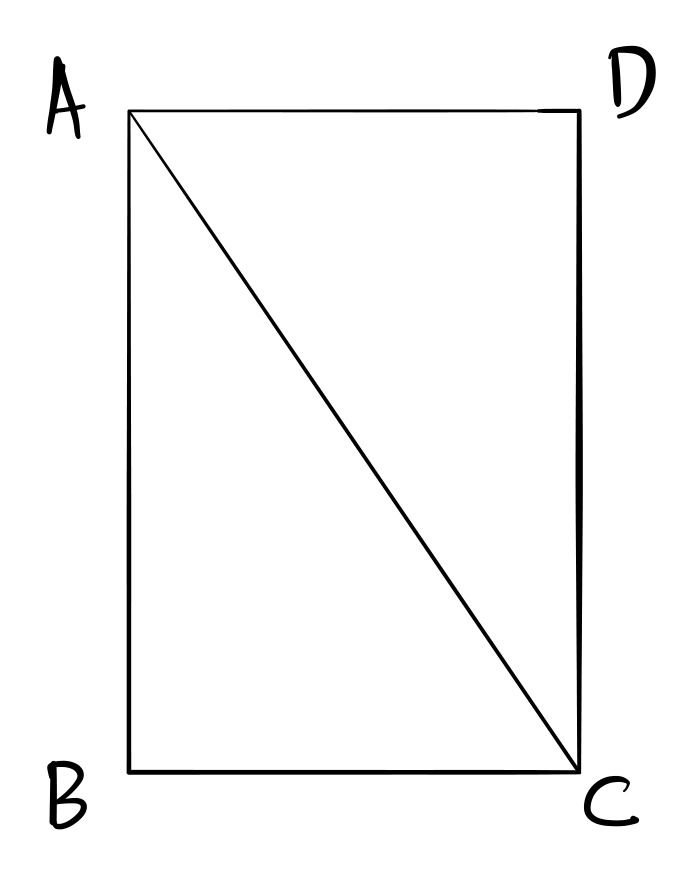
\includegraphics[scale = 0.12]{images/rect.jpeg}   
\end{center}
We want to compute the area of $\triangle ABC$, which is right angled at $B$, with $AB = h$ and $BC = b$. We enclose it within the closed rectangle $ABCD$, whose area is $length(AB).length(BC) = bh$ (from \textbf{P3}). 

Now $area(\triangle ABC) = area(\triangle ADC)$ (because $\triangle ADC$ is the rotation of $\triangle ABC$ about midpoint of $AC$, hence the area remains the same).

Now, let $P$ denote $\triangle ABC$ and let $Q$ denote $\triangle ADC$ and $R$ denote rectangle $ABCD$. Let $\chi_P$, $\chi_Q$ and $\chi_R$ denote respective characteristic functions with respect to $R$.

Clearly, $\chi_R = \chi_P + \chi_Q - \chi_{AC} \implies area(R) = area(P) + area(Q) - \int_{R} \chi_{AC}$. Now, $AC$ is a line segment with content zero, hence has area $0$. This mean $area(R) = area(P) + area(Q) \implies area(R) = 2.area(P) \implies area(P) = area(\triangle ABC) = \frac{area(R)}{2} = \frac{bh}{2}$.

Now, for any general triangle, we drop a perpendicular to the base from the acute angled vertex (so that the altitude remains inside the triangle, dividing the triangle into $2$ right triangles, as shown in the diagram below). Let the height $PO = h$, where $PO \perp QR$ and $QO = a$ and $OR = b$. 
\begin{center}
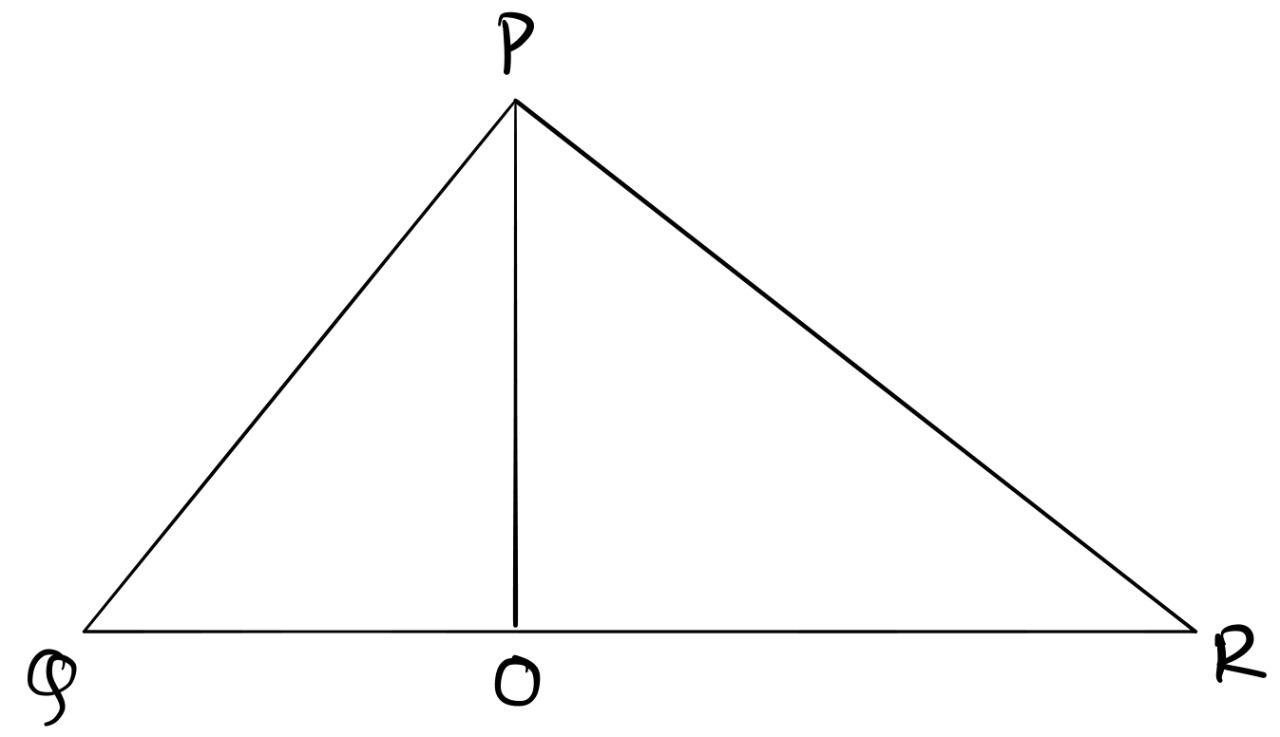
\includegraphics[scale = 0.12]{images/tri.jpeg}   
\end{center}
Now, let $\chi_0$, $\chi_1$, $\chi_2$ and $\chi_{PO}$ denote the characteristic functions of $\triangle PQR$, $\triangle PQO$, $\triangle PRO$ and $PO$ respectively with respect to a closed rectangle $R$ containing $\triangle PQR$.

So, $\chi_0 = \chi_1 + \chi_2 - \chi_{PO} \implies area(\triangle PQR)= area(\triangle PQO) + area(\triangle PRO) - \int_R \chi_{PO} \implies area(\triangle PQR)= area(\triangle PQO) + area(\triangle PRO)$.

Now, as shown previously, $area(\triangle PQO) = \frac{ah}{2}$ and $area(\triangle PRO) = \frac{bh}{2}$. So, $area(\triangle PQR) = \frac{(a+b)h}{2} = \frac{1}{2}.QR.PO$, where $PO \perp QR$.

\newpage
\item Show that the area of a closed disc of radius 1 is $\pi$. Use the formula for the area of a triangle and squeeze the disc between sets you can write down the area for. You can use any power series expression for $\pi$ that you know or can find. 

\textbf{Solution 9:}

$S = \{(x,y)|x^2+y^2 \le 1\}$, is the set of points contained in a closed disc of radius $1$.

We first show that $S$ is acceptable. $S$ is closed hence $\overline{S} = S$. $S^o = \{(x,y)|x^2+y^2 < 1\}$. So, $\partial S = \overline{S} - S^o = \{(x,y)|x^2+y^2 = 1\}$. We will show that $\partial S$ has content zero.

Let $\epsilon > 0$ be given. Now, consider this diagram.
\begin{center}
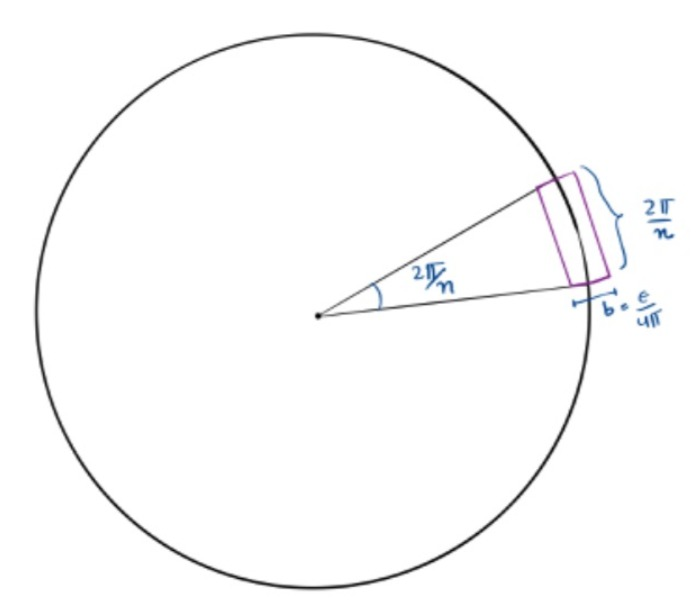
\includegraphics[scale = 0.2]{images/circ.jpeg}   
\end{center}
Here, we divide the circumference into $n$ arcs of equal length $\frac{2\pi}{n}$. When we take $n$ large enough, this arc will almost approximate to line segments of length $\frac{2\pi}{n}$. Consider, rectangles enclosing each of those parts as shown in the diagram. We take the length of each such rectangle to be $\frac{4\pi}{n}$ (so that the length of rectangle encloses the arc) and breadth to be $\frac{\epsilon}{8\pi}$. Let $R_1, R_2, ... R_n$ be the rectangles enclosing each arc.

Clearly $\partial S \subset \cup_{i = 1}^{n} R_i$. Now, we know that area of acceptable sets remains unchanged under rotation and translation. So, area of each $R_i$ is $\frac{4\pi}{n}.\frac{\epsilon}{8\pi} = \frac{\epsilon}{2n}$.

So, $\sum_{i = 1}^{n} area(R_i) = n.\frac{\epsilon}{2n} = \frac{\epsilon}{2} < \epsilon$. Hence, $\partial S$ has content zero, implying $S$ is acceptable.

In order to calculate the area of a circle, we first calculate the area of a regular polygon of $n$ sides.

Let the distance from each vertex of the polygon, to the centre of the polygon be $a$. Now, we cut the polygon into $n$, triangles, each sharing its base with the side of the polygon and having its apex vertex as the centre of the polygon.

Now, in each of these $n$ triangles, the apex angle is $\frac{2\pi}{n}$. Hence, the height of this triangle is $a \cos{\frac{\pi}{n}}$ and base $2a \sin{\frac{\pi}{n}}$. Hence, by \textbf{P8}, area of each of these triangle is $\frac{1}{2}.2a \sin{\frac{\pi}{n}}.a \cos{\frac{\pi}{n}} = \frac{a^2}{2} \sin{\frac{2\pi}{n}}$.

Now, each of these polygons are made by union of $n$ such (almost) disjoint (non-disjoint parts are just the sides of triangles, which have content zero  and don't contribute to the area) triangles.

So, area of polygon = $n$ times area of each triangle = $n.\frac{a^2}{2} \sin{\frac{2\pi}{n}} = \frac{na^2}{2} \sin{\frac{2\pi}{n}}$.

Now, to compute the area of the unit circle, we consider the following-
\begin{center}
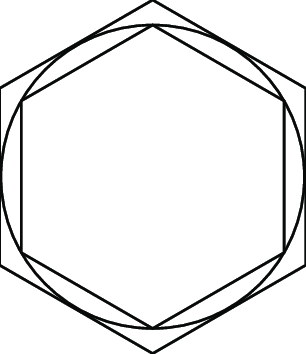
\includegraphics[scale = 0.3]{images/circle.png}   
\end{center}
We inscribe the unit circle within a regular polygon $A$ with $a = \frac{1}{\cos{\frac{\pi}{n}}}$ and we inscribe another regular polygon $B$ inside the circle with $a = 1$.

Hence, area of outer polygon $A$ as evaluated before is $n\tan{\frac{\pi}{n}}$ and similarly area of the inner polygon $B$ as evaluated before is $\frac{n}{2} \sin{\frac{2\pi}{n}}$.

Clearly, $B \subseteq S \subseteq A$. Hence, $area(B) \le area(S) \le area(A)$ (this is because, when consider the characteristic functions of each with respect to closed rectangle containing all of these $\chi_B \le \chi_S \le \chi_A$, hence follows the inequality of areas).

This means $f\forall n \ge 3$, $n\tan{\frac{\pi}{n}} \le area(S) \le \frac{n}{2} \sin{\frac{2\pi}{n}}$. Now, taking limit as $n \to \infty$, we obtain that, $\pi \le area(S) \le \pi$ (using the results $lim_{x \to 0} \frac{\sin{x}}{x} = 1$ and $lim_{x \to 0} \frac{\tan{x}}{x} = 1$). Hence, $area(S) = \pi$.

\newpage
\item As indicated in a footnote in the notes, a subset $S$ of $\bbR^2$ is \emph{Jordan measurable} if it is bounded, and for some rectangle $R \supset S$,
$\chi_S$ is measurable. It is almost the same definition as that of an acceptable set except that Jordan measurable sets need not be closed. The theory of integrable functions, integration, and area goes through as for acceptable sets. 

(See
\url{https://math.libretexts.org/Bookshelves/Analysis/Book%3A_Introduction_to_Real_Analysis_(Lebl)/11%3A_Multivariable_Integral/11.05%3A_Jordan_Measurable_Sets}.

What fails to go through? Give an easy example, starting with a Jordan measurable set that is not closed.

\textbf{Solution 10:}

Consider the set $R = [0,1] \times [0,1]$. Let $S = (0,1) \times (0,1)$. Clearly, $S \subset R$. Hence, it is bounded. Now, $\chi_S$ is Riemann integrable as for any partition $P$ of $R$, $U(P,\chi_S) = L(P,\chi_S) = area(R) = 1$. Hence, $S$ is \textit{Jordan measurable}.

Now consider a continuous function $f:S \to \bbR$, given by- $$f(x,y) = \frac{1}{xy}$$ 

Clearly when either $x$ or $y$ goes near zero, the value of $f(x,y)$ shoots up. Formally, for any $M>0$, $f(\frac{1}{\sqrt{2M}},\frac{1}{\sqrt{2M}}) = \frac{1}{\frac{1}{\sqrt{2M}}.\frac{1}{\sqrt{2M}}} = 2M > M$. Hence, $f$ is unbounded, and not Riemann integrable. Hence, a continuous function on a \textit{Jordan measurable} set $S$ is still not Riemann integrable.

\end{enumerate}



\end{document}

 